\documentclass[10pt]{standalone}
\usepackage[utf8]{inputenc}
\usepackage{pgf,tikz}
\usepackage{mathrsfs}
\usetikzlibrary{arrows,positioning,calc}
\pagestyle{empty}
\usepackage[T1]{fontenc} % font encoding
\usepackage[utf8]{inputenc} % input encoding
%\usepackage{noto}
\usepackage[largesc]{newtxtext} %
\usepackage[varqu,varl]{zi4}% inconsolata
\usepackage{cabin}% sans serif
\usepackage[vvarbb]{newtxmath}
\useosf % use oldstyle figures except in math

%\tikzset{every picture/.style={scale=0.3,every picture/.style={}}}
\tikzset{main base/.style={draw,thick,text centered, }, }
\tikzset{main node/.style={rectangle, draw,rounded corners,main base}, }
%      
%\tikzset{main verb/.style={minimum size=1cm}, }
%\tikzset{linea/.style={-triangle 90}, }
%\tikzset{main node2/.style={rectangle, draw,thick,
%    text width=7em, text centered, rounded corners, minimum height=3em}, }
\tikzset{main node2/.style={main node,
    text width=7em, minimum height=3em}, }
\tikzset{main verb/.style={minimum size=1cm}, }
\tikzset{linea/.style={-triangle 90,thick,draw}}
%\tikzset{linea/.style={-triangle 90,thick,draw}}
\tikzset{linea2/.style={-triangle 90,draw}}
\tikzset{primo/.style={circle,draw,inner sep=0pt,minimum size=1pt,thick}, }
\tikzset{
    start-end/.style={
        draw,
        rectangle,
        rounded corners,main base,
    } ,
    input/.style={ % requires library shapes.geometric
        draw,
        trapezium,
        trapezium left angle=60,
        trapezium right angle=120,main base
    },
    operation/.style={
        draw,thick,
        rectangle,main base,
    },
    loop/.style={ % requires library shapes.misc
        draw,
        chamfered rectangle,
        chamfered rectangle xsep=2cm
    },
    decision/.style={ % requires library shapes.geometric
        draw,
        diamond,
        aspect=#1,main base
    },
    decision/.default=1,
    print/.style={ % requires library shapes.symbols
        draw,
        tape,
        tape bend top=none
    },
    connection/.style={
        draw,
        circle,
        radius=5pt,
    },
    process rectangle outer width/.initial=0.15cm,
    predefined process/.style={
        rectangle,
        draw,
        append after command={
        \pgfextra{
          \draw
          ($(\tikzlastnode.north west)-(0,0.5\pgflinewidth)$)--
          ($(\tikzlastnode.north west)-(\pgfkeysvalueof{/tikz/process rectangle outer width},0.5\pgflinewidth)$)--
          ($(\tikzlastnode.south west)+(-\pgfkeysvalueof{/tikz/process rectangle outer width},+0.5\pgflinewidth)$)--
          ($(\tikzlastnode.south west)+(0,0.5\pgflinewidth)$);
          \draw
          ($(\tikzlastnode.north east)-(0,0.5\pgflinewidth)$)--
          ($(\tikzlastnode.north east)+(\pgfkeysvalueof{/tikz/process rectangle outer width},-0.5\pgflinewidth)$)--
          ($(\tikzlastnode.south east)+(\pgfkeysvalueof{/tikz/process rectangle outer width},0.5\pgflinewidth)$)--
          ($(\tikzlastnode.south east)+(0,0.5\pgflinewidth)$);
        }  
        },
        text width=#1,
        align=center
    },
    predefined process/.default=1.75cm,
    man op/.style={ % requires library shapes.geometric
        draw,
        trapezium,
        shape border rotate=180,
        text width=2cm,
        align=center,
    },
    extract/.style={
        draw,
        isosceles triangle,
        isosceles triangle apex angle=60,
        shape border rotate=90
    },
    merge/.style={
        draw,
        isosceles triangle,
        isosceles triangle apex angle=60,
        shape border rotate=-90
    },
}

\begin{document}
  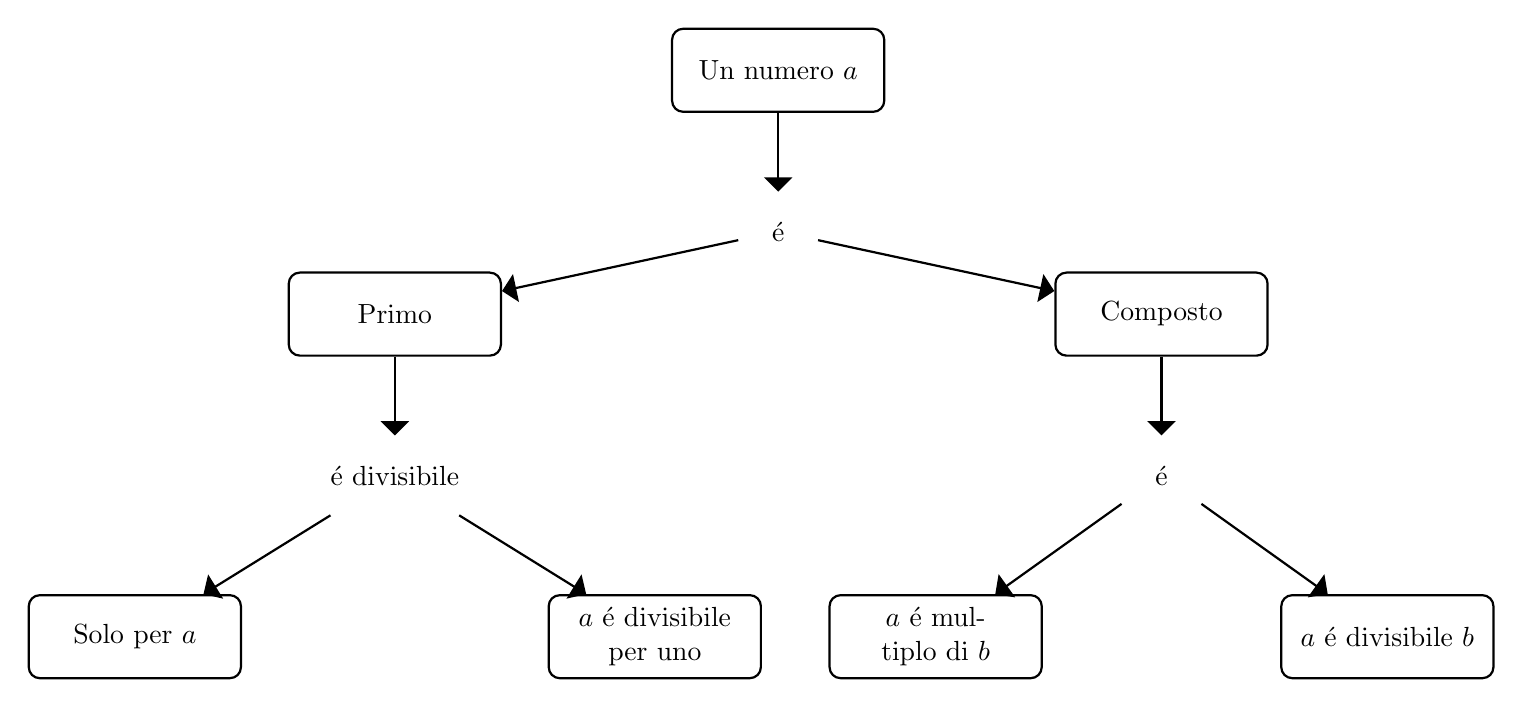
\begin{tikzpicture}
  \tikzset{every picture/.style={scale=0.3,every picture/.style={}}}
  \tikzset{main base/.style={draw,thick,text centered, }, }
  \tikzset{main node/.style={rectangle, draw,rounded corners,main base}, }
  %      
  %\tikzset{main verb/.style={minimum size=1cm}, }
  %\tikzset{linea/.style={-triangle 90}, }
  %\tikzset{main node2/.style={rectangle, draw,thick,
  %    text width=7em, text centered, rounded corners, minimum height=3em}, }
  \tikzset{main node2/.style={main node,
  		text width=7em, minimum height=3em}, }
  \tikzset{main verb/.style={minimum size=1cm}, }
  \tikzset{linea/.style={-triangle 90,thick,draw}}
  %\tikzset{linea/.style={-triangle 90,thick,draw}}
  \tikzset{linea2/.style={-triangle 90,draw}}
  \tikzset{primo/.style={circle,draw,inner sep=0pt,minimum size=1pt,thick}, }
  \tikzset{
  	start-end/.style={
  		draw,
  		rectangle,
  		rounded corners,main base,
  	} ,
  	input/.style={ % requires library shapes.geometric
  		draw,
  		trapezium,
  		trapezium left angle=60,
  		trapezium right angle=120,main base
  	},
  	operation/.style={
  		draw,thick,
  		rectangle,main base,
  	},
  	loop/.style={ % requires library shapes.misc
  		draw,
  		chamfered rectangle,
  		chamfered rectangle xsep=2cm
  	},
  	decision/.style={ % requires library shapes.geometric
  		draw,
  		diamond,
  		aspect=#1,main base
  	},
  	decision/.default=1,
  	print/.style={ % requires library shapes.symbols
  		draw,
  		tape,
  		tape bend top=none
  	},
  	connection/.style={
  		draw,
  		circle,
  		radius=5pt,
  	},
  	process rectangle outer width/.initial=0.15cm,
  	predefined process/.style={
  		rectangle,
  		draw,
  		append after command={
  			\pgfextra{
  				\draw
  				($(\tikzlastnode.north west)-(0,0.5\pgflinewidth)$)--
  				($(\tikzlastnode.north west)-(\pgfkeysvalueof{/tikz/process rectangle outer width},0.5\pgflinewidth)$)--
  				($(\tikzlastnode.south west)+(-\pgfkeysvalueof{/tikz/process rectangle outer width},+0.5\pgflinewidth)$)--
  				($(\tikzlastnode.south west)+(0,0.5\pgflinewidth)$);
  				\draw
  				($(\tikzlastnode.north east)-(0,0.5\pgflinewidth)$)--
  				($(\tikzlastnode.north east)+(\pgfkeysvalueof{/tikz/process rectangle outer width},-0.5\pgflinewidth)$)--
  				($(\tikzlastnode.south east)+(\pgfkeysvalueof{/tikz/process rectangle outer width},0.5\pgflinewidth)$)--
  				($(\tikzlastnode.south east)+(0,0.5\pgflinewidth)$);
  			}  
  		},
  		text width=#1,
  		align=center
  	},
  	predefined process/.default=1.75cm,
  	man op/.style={ % requires library shapes.geometric
  		draw,
  		trapezium,
  		shape border rotate=180,
  		text width=2cm,
  		align=center,
  	},
  	extract/.style={
  		draw,
  		isosceles triangle,
  		isosceles triangle apex angle=60,
  		shape border rotate=90
  	},
  	merge/.style={
  		draw,
  		isosceles triangle,
  		isosceles triangle apex angle=60,
  		shape border rotate=-90
  	},
  }
    \node[main node2] (1) {Un numero $a$};
    \node[main verb] (2) [below = of 1]  {\'{e}};
  
    \node[main node2] (3) [below right=0cm and 3 cm of 2]  {Composto};
    \node[main node2] (4) [below left=0cm and 3 cm of 2]  {Primo};
    
    \node[main verb] (5) [below =of 4]  {\'{e} divisibile};
    \node[main verb] (6) [below =of 3]  {\'{e} };
    
     \node[main node2] (7) [below left=of 5]  { Solo per $a$};
     \node[main node2] (8) [below right=of 5]  {$a$ \'{e} divisibile per uno};
     
     \node[main node2] (9) [below left=of 6]  {$a$ \'{e} multiplo di $b$};
     \node[main node2] (10) [below right=of 6]  {$a$ \'{e} divisibile $b$};
\foreach \x /\y in{1/2,2/3,2/4,4/5,3/6,5/7,5/8,6/9,6/10}
  \path[linea] (\x) edge node {} (\y);
%  
\end{tikzpicture}
\end{document}